% figures.tex


\begin{figure}[h]
    \centering
    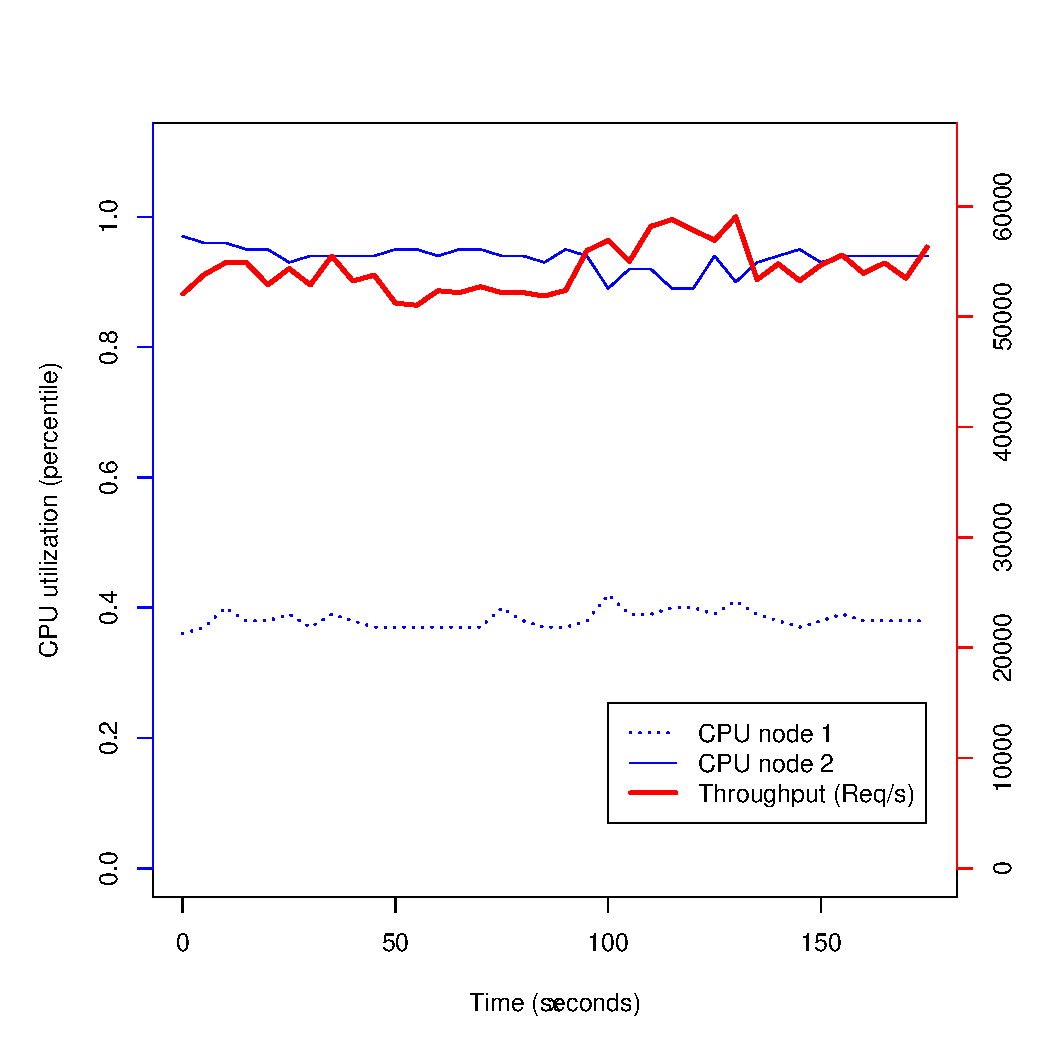
\includegraphics[width=1.2\textwidth]{results/baseline_originalsrc_v182}
    \caption{Baseline for original source code. 2 heterogeneous Nodes, 8 partitions each.}
    \label{fig:baseline}
\end{figure}

\begin{figure}[h]
    \centering
    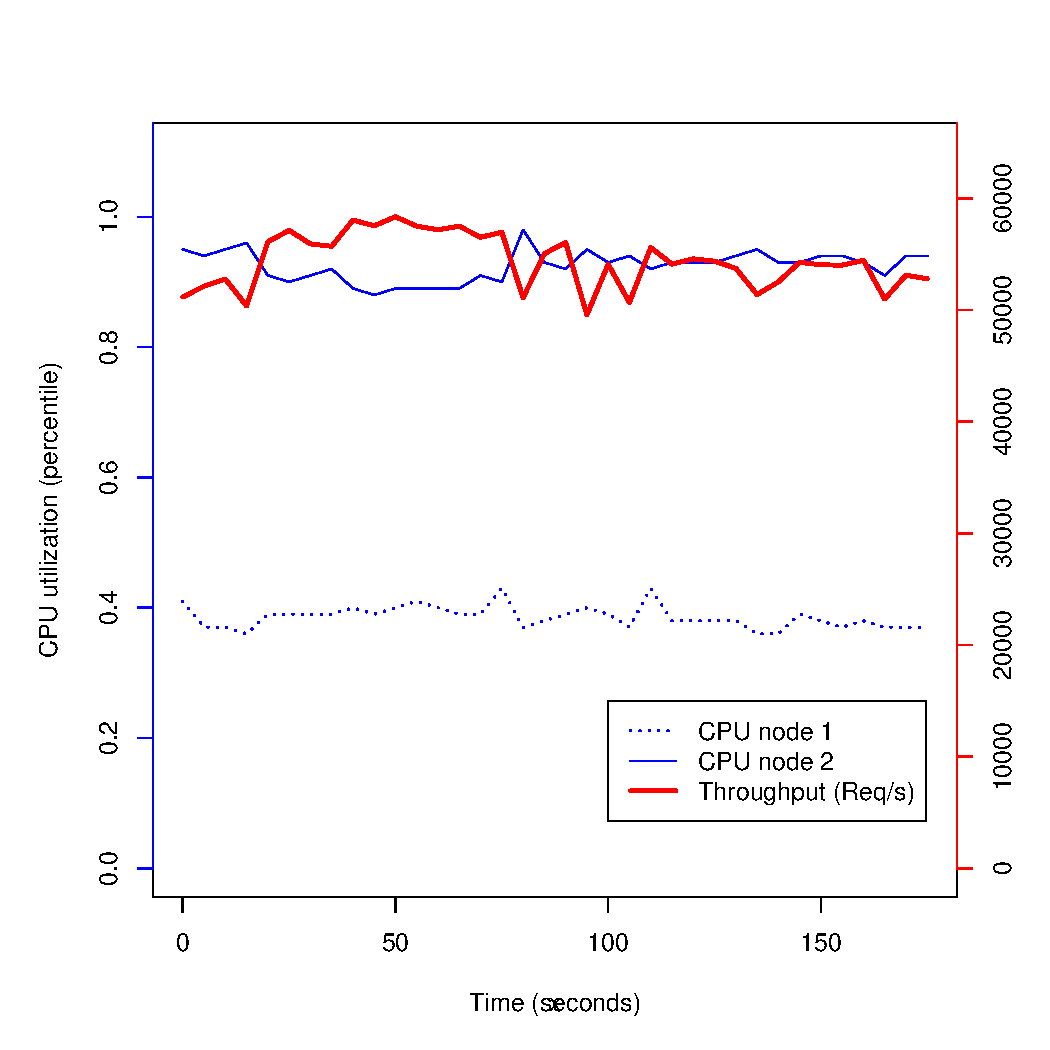
\includegraphics[width=1.2\textwidth]{results/baseline_plot}
    \caption{Baseline for our modified source. 2 heterogeneous nodes, 8 partitions each.}
    \label{fig:baseline}
\end{figure}

\begin{figure}[h]
    \centering
    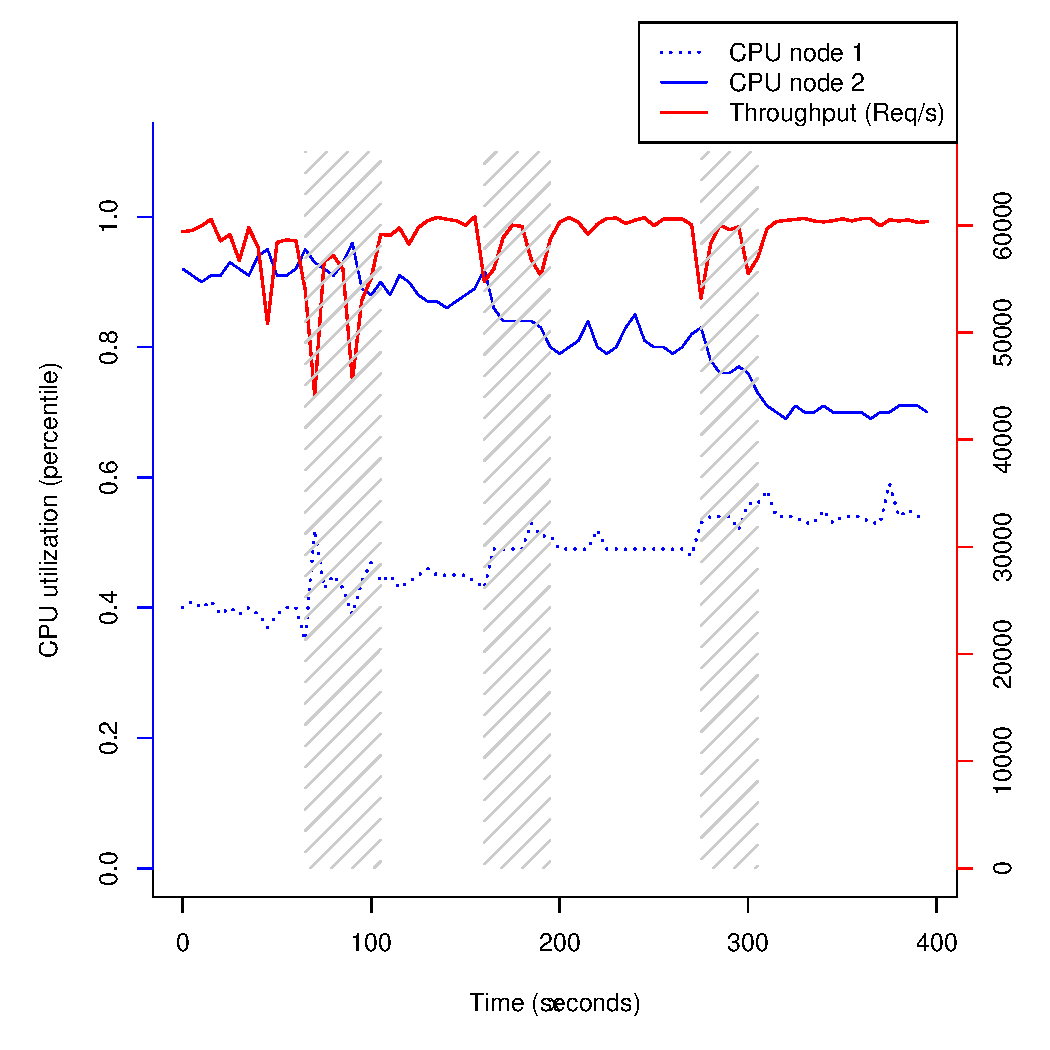
\includegraphics[width=1.2\textwidth]{results/rebalance_originalsrc}
    \caption{Manual moving of 3 partitions from a struggling node (Node 2). Grey regions mark rebalance period, where data is prepared and transferred between nodes.}
    \label{fig:adaptive}
\end{figure}

\begin{figure}[h]
    \centering
    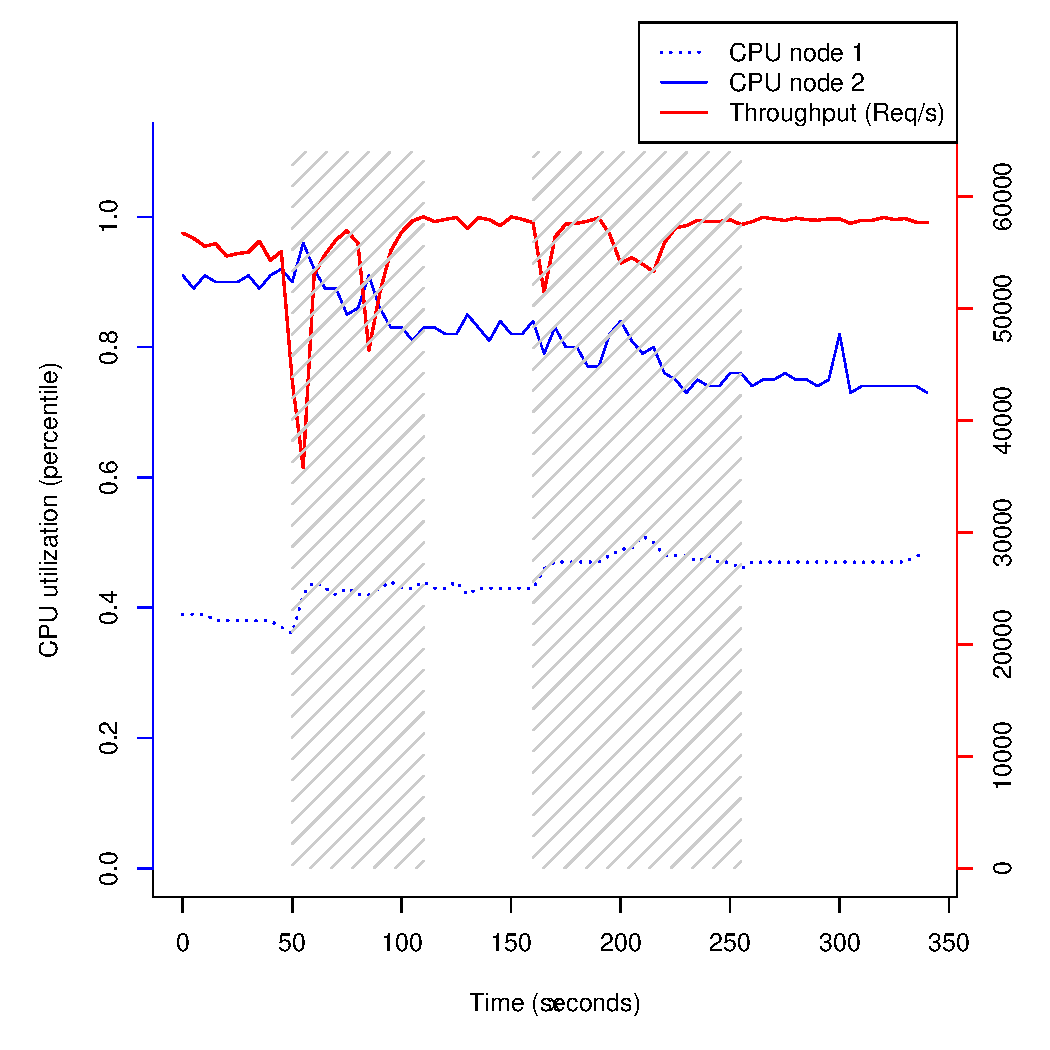
\includegraphics[width=1.2\textwidth]{results/adaptive_plot}
    \caption{Automatic moving of 2 partitions from a struggling node (Node 2). Grey regions mark rebalance period, where data is prepared and transferred between nodes. CPU threshold set at \texttt{0.8}.}
    \label{fig:adaptive}
\end{figure}

